% ---------------------------------------------
%
%   __ _ _ __ ___  __ _
%  / _` | '__/ _ \/ _` | /\/|
% | (_| | | |  __/ (_| ||/\/
%  \__,_|_|  \___|\__,_|
% ---------------------------------------------
%*[ ]   Create Github Page
%*[ ]   Re-draft
%*[ ]   Link to theory
%*[ ]   Link to design patterns
% ---------------------------------------------
\chapter{Composing area\textasciitilde{}}{Exploring Real and Virtual Environments Through Gestural Ambisonics and Audio Augmented Reality}
\label{sec: area}
\markboth{}{Composing area\textasciitilde{}: Exploring Real and Virtual Environments Through Gestural Ambisonics and Audio Augmented Reality}
\epigraph{\emph{This chapter draws the majority of its content from a published article in the Goldsmith's journal \textit{Sonic Scope: New Approaches to Audiovisual Culture}}}{\citep[]{bilbow2021a}}
% ---------------------------------------------
%\section{Abstract}                              \label{sec: area-abstract}
%In this paper, I outline the development and evaluation of the \textit{area\textasciitilde{}} system. \textit{area\textasciitilde{}} enables users to record, manipulate, and spatialise virtual audio samples or nodes around their immediate environment. Through a combination of ambisonics audio rendering and hand gesture tracking, this system calls attention to the ability of non-visual augmented reality (AR), here, audio augmented reality (AAR), to provide new aesthetic experiences of real and virtual environments. The system is contextualised within the move in computational art, and indeed, broader human computer interaction research, towards multisensory interaction. In particular, \textit{area\textasciitilde{}} is situated in the creative practice of works using multisensory AR as a medium to create expressive computational art.

%Through an autobiographical design study, these experiences are discussed in relation to the research question: \textit{“How can we better understand relationships between virtual and real environments through gesture and virtually placed audio augmented reality objects?”} This hypothesis study proposes that new aesthetic experiences can result from the system and are waiting to be tested through user studies. The adoption of the Project North Star open-source AR head-mounted-display (HMD) could expand the possibilities of the \textit{area\textasciitilde{}} system by reducing the need to be tethered to a laptop and table for hand gesture input.

%In discussing the future development of the system and my research, I propose a devising practice-led method for creating and evaluating new multisensory AR (MSAR) Experiences; as well as the tantalising prospect of adding interaction between other sensory modalities to the \textit{area\textasciitilde{}} system, such as vision or smell, which would be made possible by the use of this open-source HMD.

% ---------------------------------------------
%\section{Introduction}                          \label{sec: area-intro}
%An augmented reality (AR) system is widely accepted as a system that utilises the combination of “real and virtual”, is interactive in real-time, and registered in three dimensions \citep{azuma1997}. Although this definition entertains the prospect of multisensory applications, in the last twenty years, the vast majority of AR applications have dealt with visual displays of information \citep{billinghurst2015, schraffenberger2016}. Indeed, a systematic review from 2018 found that 96\% of AR usability studies conducted between 2005-2014 augmented only the visual sense \citep{dey2018}. In cross-modality psychology research, this ocularcentrism (the perceptual and epistemological bias ranking vision over other senses \citep{oxfordreference2020}) is normally explained by a ‘textbook’ explanation: “the idea that vision is the most important modality is supported by numerous studies demonstrating visual dominance”. Hutmacher \citeyearpar{hutmacher2019} argues that ocularcentrism can be critiqued through the lenses of:
%\begin{enumerate}
%    \item A methodological-structural explanation: “research on vision is often easier than research on other modalities and that this is the result of an initial bias toward vision that reinforces itself”.
%    \item A cultural explanation: “the dominance of the visual is not a historical constant, but rather a result of the way (Western) societies are designed”.
%\end{enumerate}
%Within computational arts and specifically within the composition of works using AR as their medium, ocularcentrism has been met in recent years with a push towards multisensory interaction methods \citep{billinghurst2015, schraffenberger2016,papagiannis2014,kiefer2018}. Meanwhile, within HCI research we have seen the same general movement through the development of applications and studies with multisensory interaction methods.

%Within AR and virtual reality (VR) technologies, the trend of ocularcentrism is compounded by the dominance in development of visual head-mounted-displays (HMDs). There has been an increase in the popularity and development of virtual reality HMDs, such as the Cosmos / Vive (HTC 2020), Quest 2 (Oculus 2020), and Index (Valve 2019). Augmented reality has seen its own parallel surge in development of HMDs; these include the Magic Leap 1 (Magic Leap 2018), Nreal Light (Nreal 2020), and Microsoft’s Hololens 2 (Microsoft 2019). As well as being primarily visual devices, these AR HMDs are generally expensive, in the range of £1000 - £2,500. Both VR and AR HMDs often require development licences, being locked into certain software frameworks, and provision of personal data to parent companies such as Facebook, HTC, and Microsoft.

%Alternatives to these closed-source AR offerings are possible in the form of DIY microcontroller-based solutions like the one described in this paper. Furthermore, Leap Motion; a hand tracking device company that recently merged with Ultrahaptics, open-sourced their Project North Star AR HMD designs in 2018. These are 3D printable and require approximately £300 - £400 of electronics to get started \citep{leapmotion2018}.

%This move has helped democratise the use of AR as a medium, tool, and collaborative technology, allowing the maker community develop tools \citep{rompapas2020} that aid in critiquing the tensions and various relationships between real and virtual environments. Furthermore, it has presented a unique opportunity for computational artists and digital media researchers that want to develop for an AR HMD but either cannot afford to spend £1000-£2500 on one, or cannot justify buying closed-source devices due to clashes in research ethics due the provision of personal data required by parent companies.

\section{Computational 'ARt' with \textit{area\textasciitilde{}}} \label{sec: area-intro-area}
This paper contributes towards the holistic development of AR applications by exploring one of the main attributes of an AR system: the combinational relationship of real and virtual environments, specifically within audio augmented reality (AAR). In doing so, I attempt to form a deeper understanding of AR's aesthetic and material capabilities as an artistic medium.

The \textit{area\textasciitilde{}} system is a gestural sound sampler that uses hand and head tracking to place and manipulate virtual audio sources in the user’s environment, heard through bone conduction headphones which transmit sound directly to the cochlear without occluding the user’s hearing. This allows the user to experience \textit{virtual audio environments} overlaid seamlessly onto the \textit{real audio environment}. Through gesture, the user can interact with and shape the combined \textit{real and virtual audio environment} surrounding them.

This paper will address the research question: \textit{“How can we better understand relationships between virtual and real environments through gesture and virtually placed AAR objects?”}. Understanding these relationships allows for the facilitation of engaging experiences within computational arts through richer multisensory human-computer interaction.

\subsection{Technologies}                       \label{sec: area-intro-tech}
The three technologies used in \textit{area\textasciitilde{}} are gestural hand tracking, rotational head tracking, and ambisonics. The gestural hand tracker used in the system is a Leap Motion LM-010 Controller, a USB infrared camera device that provides location and orientation data output of individual finger joints (and therefore hands) when they are presented above the device. The Leap Motion Controller (LMC) has been adopted in a multitude of settings such as being mounted on VR headsets \citep{leapmotion2016}, and converting hand gestures to MIDI (Leap Motion 2017). More recently, UltraLeap are investigating the use of this same technology with gesture-based public information screens to help combat the “hygiene risks of touch screens” \citeyearpar{ultraleap2020a}.

Rotational head tracking is achieved via an inertial measurement unit (IMU). This small and inexpensive component provides orientational data output at 20 times a second. When affixed to the head via a headset or headphones, it is a relatively easy and cheap way of implementing head tracking into the system.

Ambisonics is an audio format that allows for full-spherical audio capture and playback \citep{gerzon1973}, meaning that it includes sound sources above and below the listener as well as the conventional horizontal plane. There are four recorded channels (referred to as A-Format) that, unlike regular mono, stereo or surround sound formats, contain no information about the speakers that the signal should be delivered to. Rather, these channels can be encoded in such a way as to describe a three-dimensional field of sound referred to as B-Format, allowing the producer or artist to think in terms of sound sources in three dimensions rather than conventional speaker placement. B-Format can be decoded through “virtual microphones”, any number of which can be placed within this three-dimensional sound field to provide standard channel outputs.

For example, in \textit{area\textasciitilde{}}, I have used a RØDE Soundfield NTSF-1 microphone array comprised of 4 microphones. The A-Format output is encoded to B-Format by an audio plugin. A software library decodes the B-Format to two responsive, binaural, virtual audio output channels. This all occurs in real-time, so that the microphones inside the three-dimensional sound field rotate proportionally as the user moves their head, providing realistic changes to what is heard.


% ---------------------------------------------
%\section{Literature Review}                     \label{sec: area-literature}
%\subsection{Augmented Reality}                  \label{sec: area-literature-ar}
%Augmented reality was first defined by Caudell and Mizell in the field of aeronautical research as technology used to “augment the visual field of the user with information necessary in the performance of the current task” \citeyearpar{caudell1992}, reflecting the ongoing tendency for AR to focus on augmenting the visual rather than taking a multi-sensory approach. This paper focused on increasing the efficiency of manufacturing workers using a head-mounted display (HMD) with registration systems such as head-position tracking. Further conceptualisation came a year later when Rosenberg \citeyearpar{rosenberg1993} concluded that overlaying audio-visual information in the form of “virtual fixtures” could increase teleoperator performance by reducing demands on “taxed sensory modalities” and aiding in a perceptual simplification of the workplace. In their seminal 1994 paper, Milgram and Kishino conceptualised the “virtuality continuum”, a spectrum of ‘mixed reality' (MR) scenarios into which most, if not all, of today’s AR/VR applications and devices fit \citeyearpar{milgram1994}.
%
%From the late 1990s, AR has been defined as a technology that fits three specifications outlined by Azuma \citeyearpar{azuma1997}:
%\begin{enumerate}
%    \item Combines real and virtual
%    \item Interactive in real-time
%    \item Registered in 3-D
%\end{enumerate}
%\begin{figure}
%    \centering
%    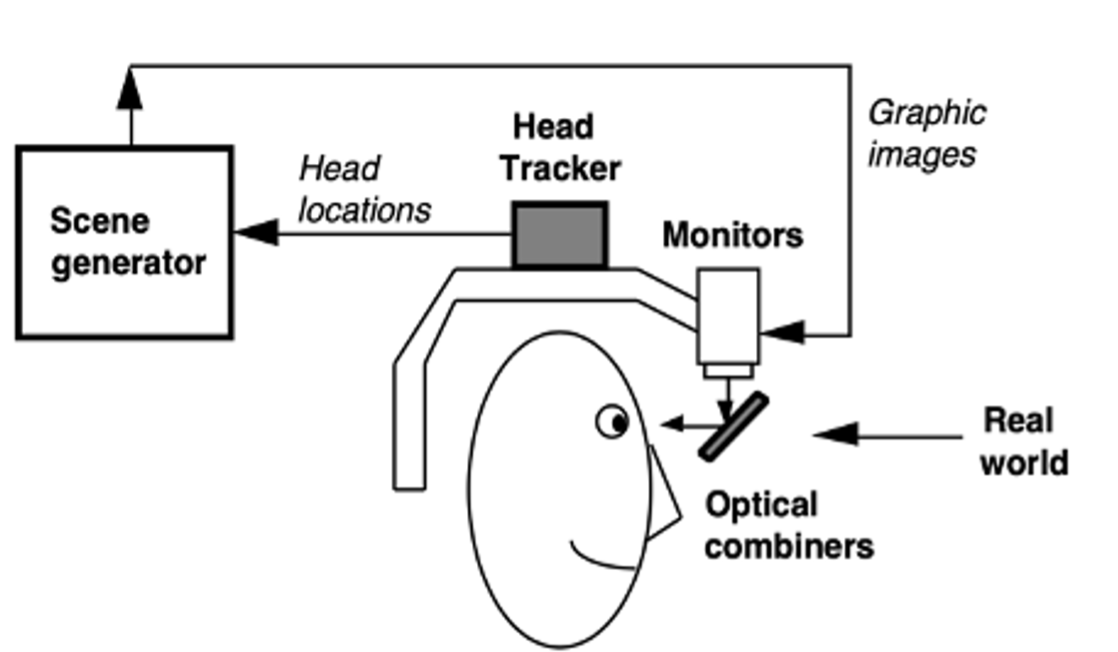
\includegraphics{figures/05-area/azuma1997_1.png}
%    \caption{Optical see through \citep{azuma1997}}
%    \label{fig: azuma1997headset}
%\end{figure}
%The paper also contains an extensive survey of existing AR applications and devices of the time, from industries as disparate as military aircraft, entertainment, and robot path-planning. Most of these applications use either HMD “optical see-through” (\autoref{fig: azuma1997headset}), or “video see-through” - “combining a closed-view HMD with one or two head-mounted video cameras” – again reflecting the understanding of AR as a primarily visual technology. 
%
%\subsection{Multisensory AR}                    \label{sec: area-literature-msar}
%AR has seen a recent surge in development, not only through the release of new HMDs (optical see-through), but also through the introduction of (video see-through) mobile AR frameworks \citep{apple2020,google2020,vuforia2020}, resulting in its use in disciplines from neuroscience \citep{mcduff2017} to the arts \citep{eliasson2020}. Most of these developments continue to approach VR via a conventional ocular-centric approach. However, following Lindeman and Noma’s \citeyearpar{lindeman2007} taxonomy of ‘multi-sensory AR’ (the use of more than one sensory overlay), the concept of multi-sensory AR has become an increasingly popular topic of discussion \citep{billinghurst2015,schraffenberger2016,papagiannis2014}. Chevalier and Kiefer \citeyearpar{chevalier2018} argue that AR should be seen as “inseparable from a multisensory ecosystem” rather than consisting only of a visual overlay, and that it is inhabited by “modes of sensing, modes of perceptual mediation, computational relationships between sensing and mediation, human participants, and their environment”. Viewing AR from a fundamentally “experience-focused and conceptual perspective”, Schraffenberger identifies ocularcentrism as an issue in AR research and practice and suggests that new perspectives on the medium must be considered in order to “inspire and facilitate new and different forms of both AR and AR research”, one of which is the investigation into “multimodal and interactive environments” \citeyearpar{schraffenberger2018}.

%\subsection{Examples of MSAR}                   \label{sec: area-literature-msarexamples}
%Some examples of experience-driven multisensory applications of AR include ‘Augmented Reality Flavours’ \citep{narumi2011}, which details the creation of a pseudo-gustatory AR interface by using a head-mounted olfactory pump to inject smells into the users nose whilst they eat a plain cookie to create the illusion of a flavoured cookie. This illusion is further enhanced via the visual alteration of the cookie through the HMD. An example of auditory focused AR is the sound installation study ‘Listening Mirrors', in which bone conduction headphones are used as a sensory overlay in conjunction with wearable and sculpted feedback devices for audio augmented reality: 
%\begin{quote}
%    “These headphones transmit sound directly to the [cochlear], bypassing the outer ear and ear drum, and so do not intervene in natural hearing. This allows our system to mediate the sonic environment by creating a mix of the real sound environment and digital reprocessing of the same environment, collected through the phone microphone” \citep{kiefer2018}. 
%\end{quote}
%Bone conduction headphones here serve as an aural equivalent to visual “optical see-through” devices, i.e. “hear-through” \citep{lindeman2008}. Likewise, Tikander outlines the necessary development of the aural equivalent of visual “video see-through” devices, i.e. “mic-through” \citep{lindeman2008}, in his paper positing an augmented reality audio headset \citeyearpar{tikander2008}. Somatosensory, or haptic AR interfaces have also been explored, with electrical muscle stimulation being used to add physical forces to mixed reality environments with results showing increased realism \citep{lopes2017}.
%
%In a broader human-computer interaction (HCI) context, multisensory interfacing is beginning to gain more traction, with increasing amounts of novel auditory \citep[p. 77]{barde2018}, haptic \citep{lopes2017,sheffield2016,maggioni2017,seah2015,vi2017a}, olfactory \citep{brooks2020}, and gustatory \citep{spence2015,vi2017a} applications offering rich multisensory experiences.


%\subsection{AR as a medium in computational art}    \label{sec: area-literature-arart}
%Computational art - the use of computational programming or software as a tool, performance aid, medium or collaborator to create art - has seen the use of AR as a medium since the early 2000’s. Grasset et al. presented case studies of AR art exhibitions, with the conclusion that for effective design of artworks, “the bond between the virtual and the real, established by the MR [mixed reality] concept should hold in all conditions the project could be used in” \citeyearpar{grasset2008}.
%
%More recently, Papagiannis has drawn attention to a broader multisensory view of AR in attempting to understand an aesthetic for AR applications, “AR is beginning to expand in new ways, beyond visual frames and into the full human sensorium” \citeyearpar{papagiannis2014}. In 2015, the Tate Sensorium multisensory art exhibition used novel mid-air haptic devices to augment visual art \citep{vi2017a}. The results of the included study found that multisensory experiences lead to audiences finding artwork more emotionally engaging compared to solely visual experiences.
%
%Chevalier and Kiefer highlight the nascent use of newer AR technologies by artists \citeyearpar{chevalier2020}. They argue that AR has significant potential for creative exploration, and that it is a medium for creating “new nuanced and fine-grained emergent aesthetic experiences” and define AR as “real-time computationally mediated perception”.
%
%The use of AR as a medium for the composition of computational art raises the question of what the materiality, both for user and developer, of such a digital tool or piece of software would look, sound, feel, taste or smell like. As Papagiannis highlights, “understanding the capacities of the technology and its constraints to exploit the technology to artistic use by envisioning novel applications and approaches, and developing new aesthetics and conventions beyond previous traditional forms” \citeyearpar{papagiannis2017}. 


% ---------------------------------------------
\section{The \textit{area\textasciitilde{}} system}      \label{sec: area-system}
The \textit{\textit{area\textasciitilde{}}}  system, which stands loosely for ‘augmented reality environmental audio’ aims to afford users the ability to spectromorphologically (defined by Smalley to concern spatial, temporal and textural qualities of sound \citeyearpar{smalley1997}) manipulate sounds from their environment into a \textit{virtual audio environment}. Through bone conduction headphones and head tracking, this sound field is heard in synchronicity with their actual environment. The system was created in order to explore and reveal the relationship between real and virtual environments.

%*[ ]   fix figure
\subsection{Hardware Implementation}            \label{sec: area-system-hardware}
\begin{figure}
    \centering
    \subcaptionbox*{}[.45\textwidth]{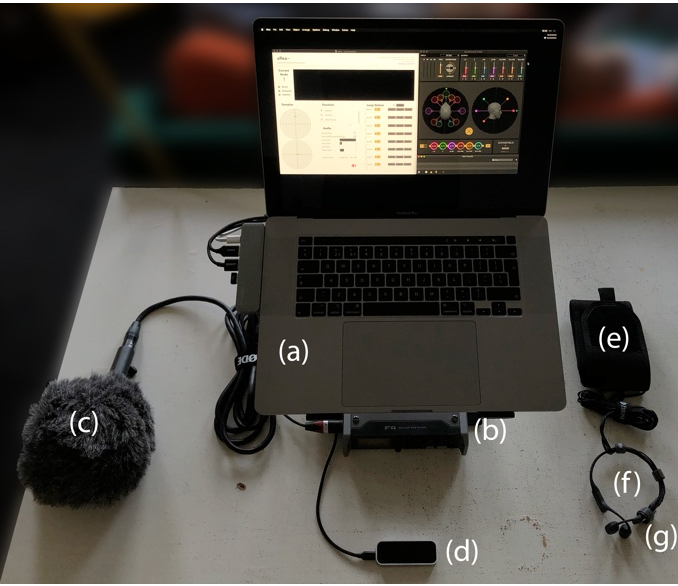
\includegraphics[height=5.5cm]{figures/05-area/areatechnical_hardware.png}}%
    \hfill
    \subcaptionbox*{}[.45\textwidth]{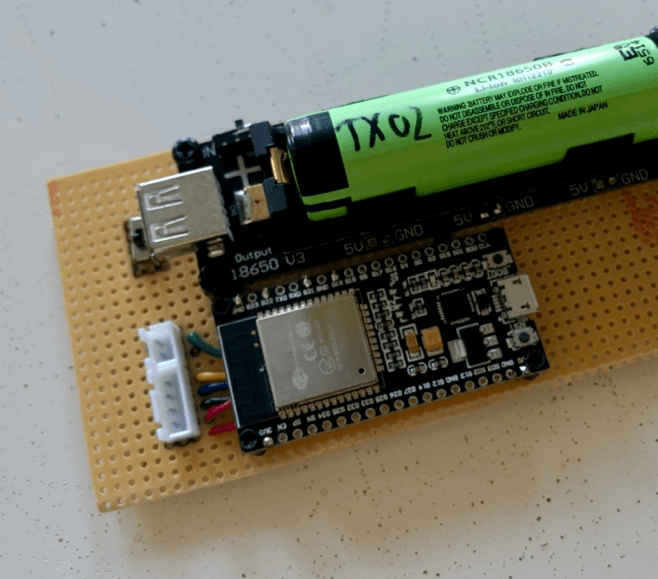
\includegraphics[height=5.5cm]{figures/05-area/areatechnical_pcb.png}}%
    \caption{\textit{area\textasciitilde{}} hardware and PCB}
    \label{fig: areatechnical}
\end{figure}

The on-desk hardware for the \textit{area\textasciitilde{}} system shown in Figure 2 includes (a) a laptop running the Max MSP \citep{cycling742020} patch, (b) a 4 channel input audio interface, (c) an Ambisonic microphone, and (d) a Leap Motion Controller \citep{ultraleap2020}.

The wearable hardware used for the \textit{area\textasciitilde{}} system comprises 2 sections: (e) a belt pouch containing a PCB-mounted ESP32 microcontroller \citep{espressif2020} and 18650 battery (shown in \autoref{fig: areatechnical}), and (f) a pair of bone conduction headphones \citep{aftershokz2020}, with (g) a mounted inertial measurement unit (IMU) for tracking head orientation. 

The IMU and ESP32 are connected via a detachable 1.5m heat shrunk cable that runs from the back of the bone conduction headphones, down the length of the user's back and into the belt-mounted transmitter pouch. With the integration of an Arduino library \citep{winer2016}, the IMU data is transmitted to the laptop via Bluetooth from the ESP32. Audio is transmitted to the headphones via Bluetooth from the Max MSP patch running on the laptop. 

The only hardware that needs to be accessible for the user is the Leap Motion Controller and the wearable hardware system. The laptop and audio interface are ideally hidden from the user. The microphone should be placed in a location that will provide the user with access to sounds that they wish to manipulate.

\subsection{Software Implementation}            \label{sec: area-system-software}

%*[ ]   fix figure
\begin{figure}
    \centering
    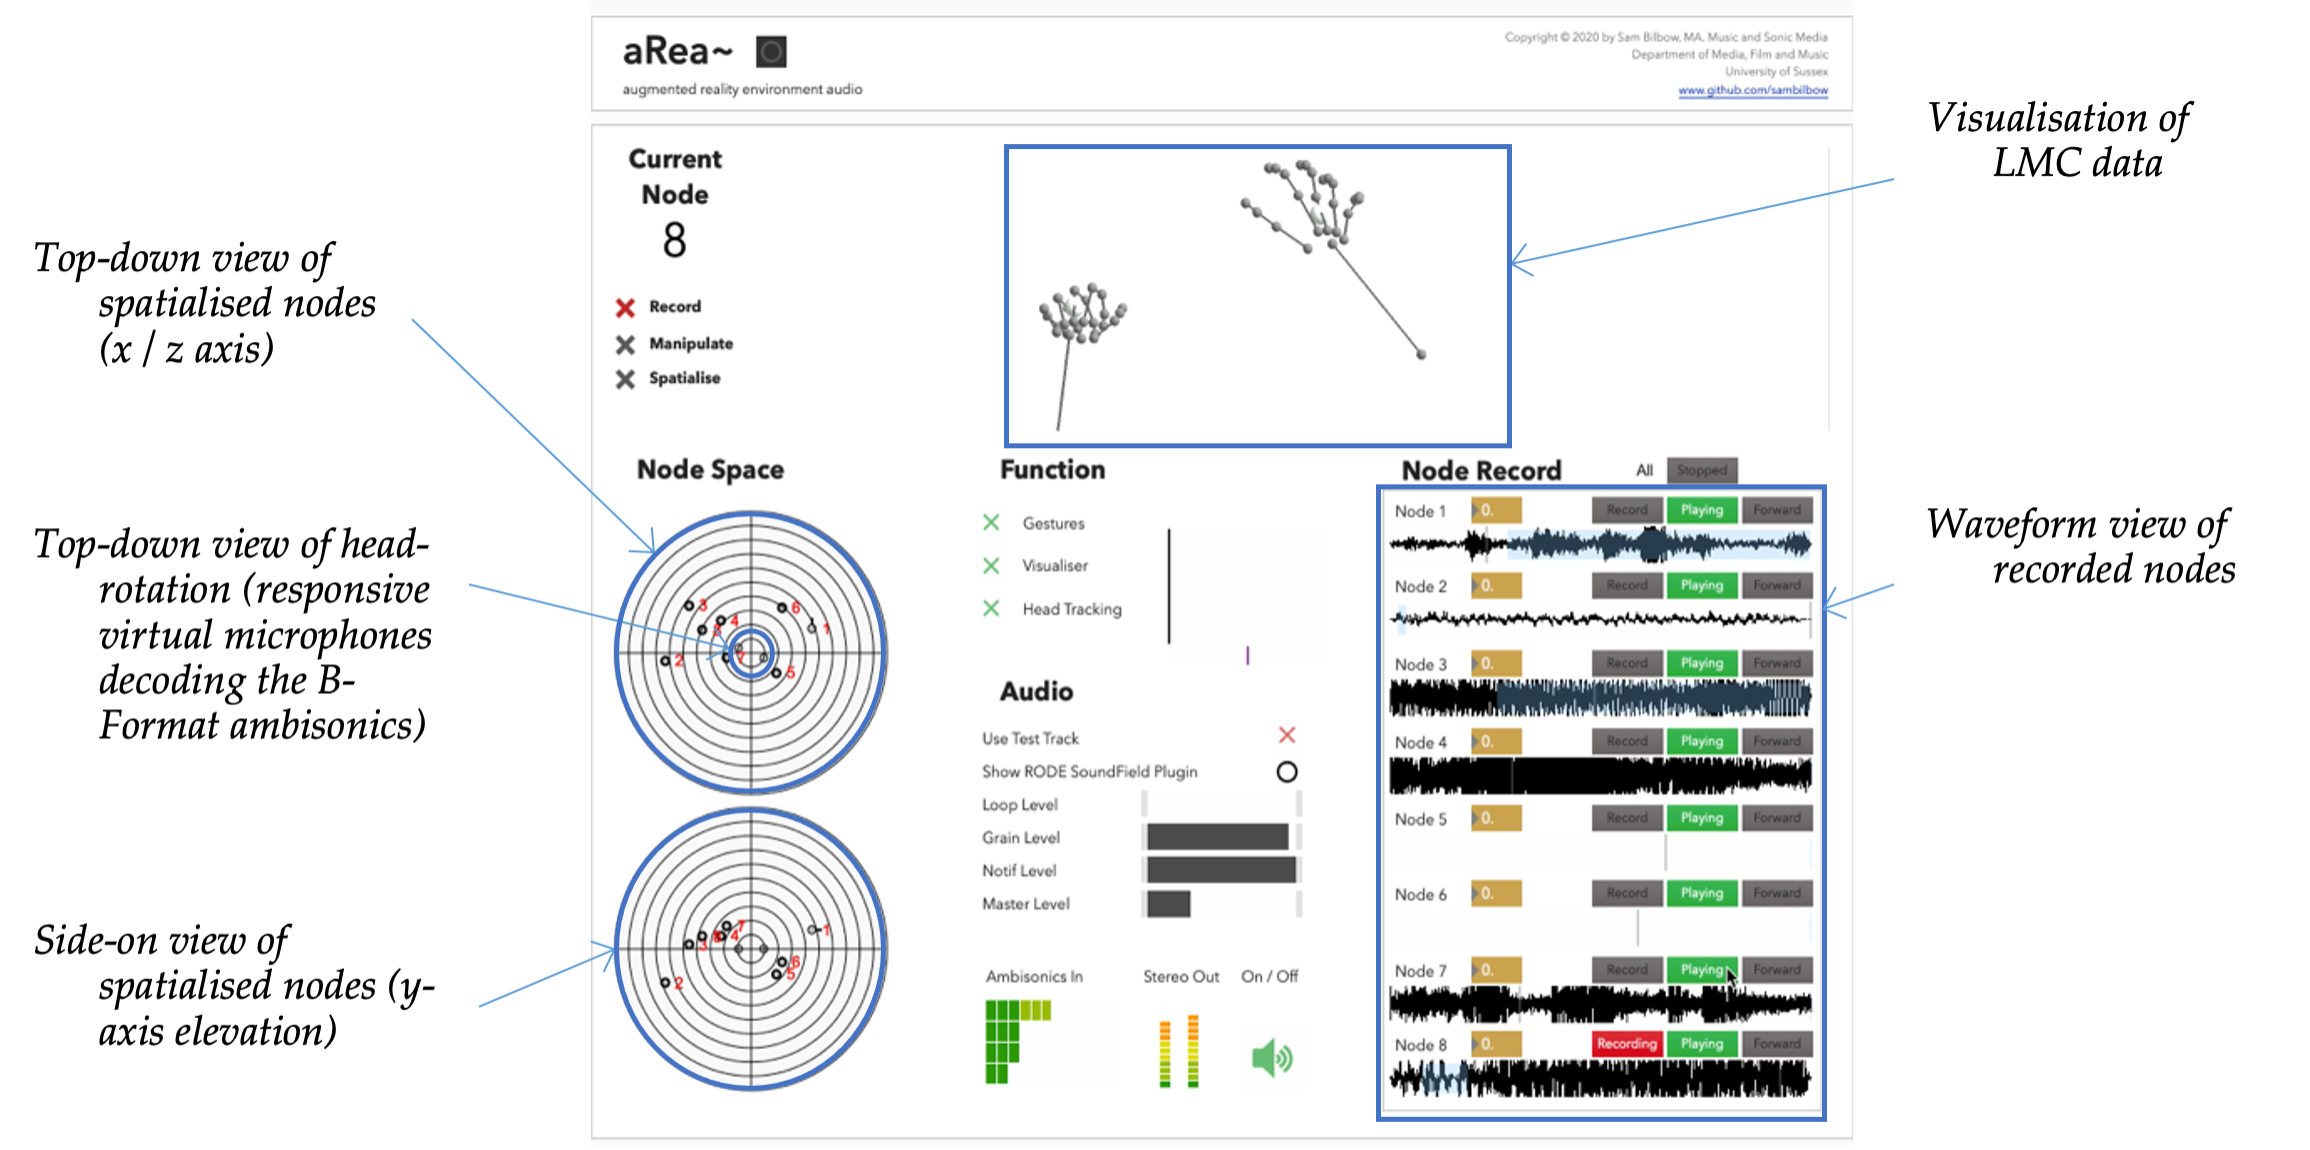
\includegraphics[width=\linewidth]{figures/05-area/areatechnical_max.png}
    \caption{\textit{area\textasciitilde{}} Max MSP patch}
    \label{fig: areatechnicalmax}
\end{figure}
The patch (\autoref{fig: areatechnicalmax}) uses the audio plugin \citep{rode2020} shown in \autoref{fig: areatechnicalrode} to encode the A-Format ambisonics microphone input into B-Format (a three-dimensional sound field), or what I will refer to as the \textit{ambisonic palette}. This \textit{ambisonic palette} is not heard by the user; instead, they can sculpt from it, forming their own audible \textit{(B-Format) virtual audio environment} through hand gestures. I have defined these gestures in Max MSP with help from the IRCAM Leap Motion library \citeyearpar{ircam2014}, and they occur over three stages of user interaction: \textit{\textbf{record, manipulate, spatialise}}. 

%*[ ]   fix figure
\begin{figure}
    \centering
    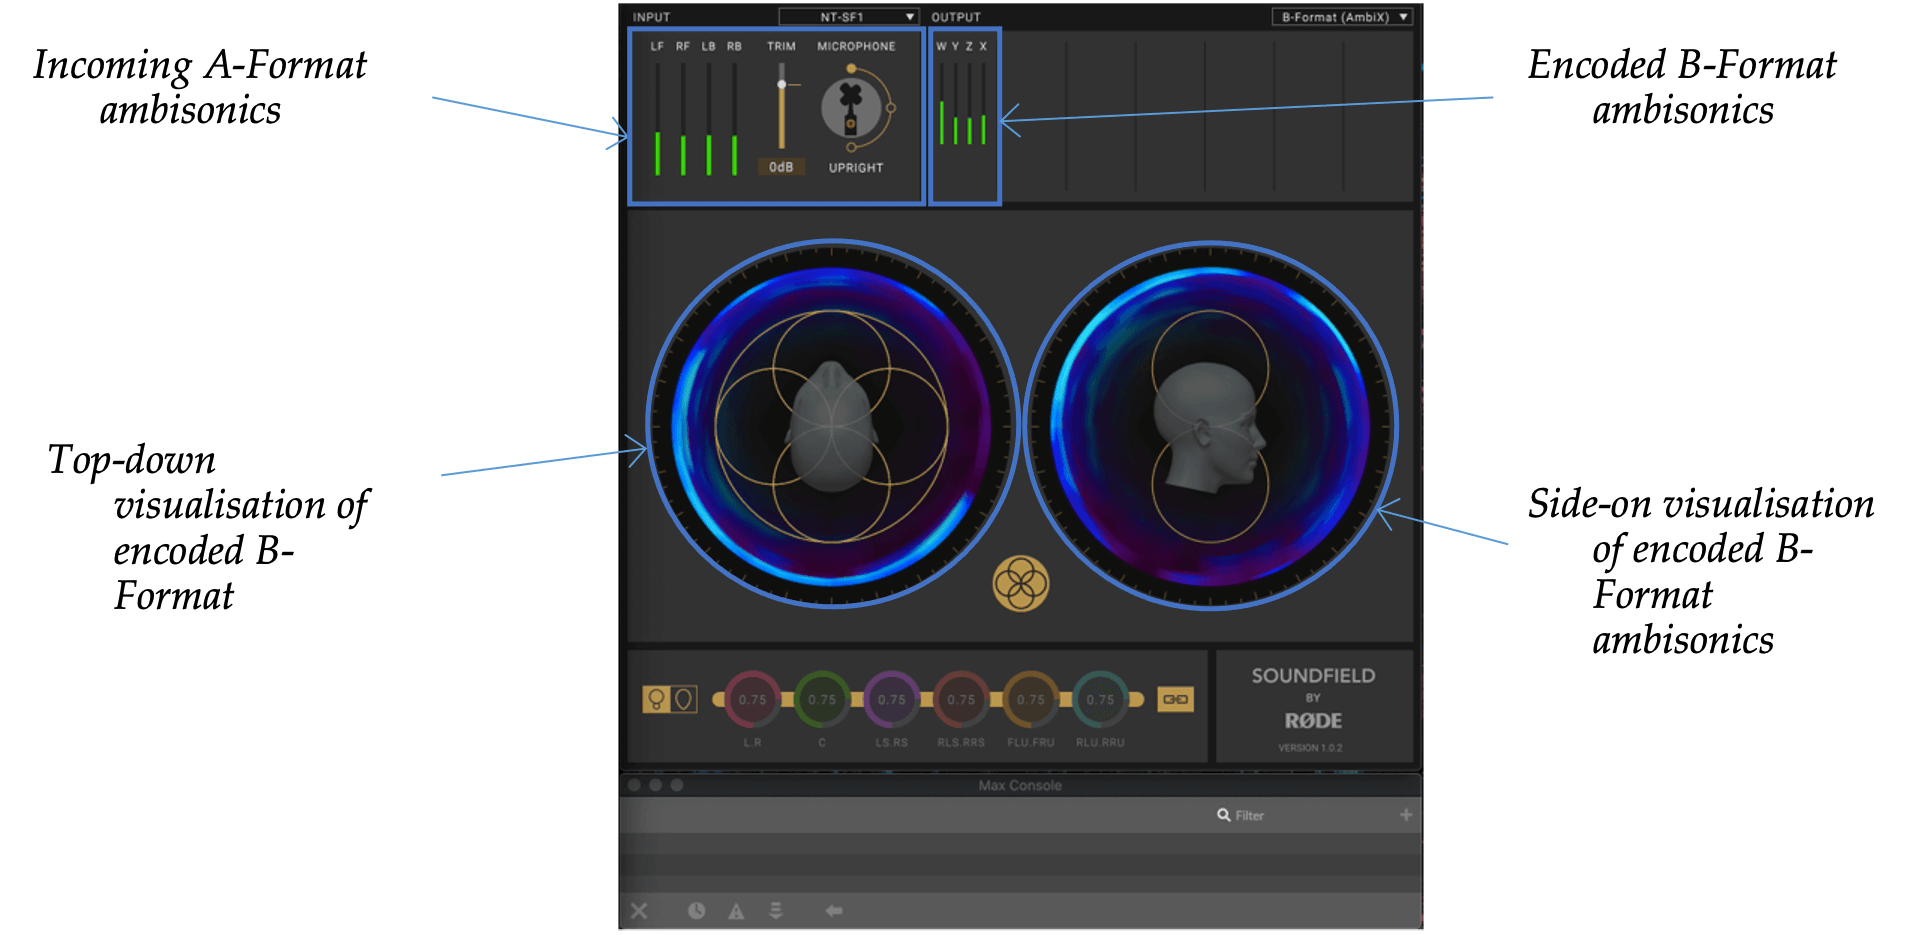
\includegraphics[width=\linewidth]{figures/05-area/areatechnical_rode.png}
    \caption{RØDE Soundfield Plugin}
    \label{fig: areatechnicalrode}
\end{figure}

\subsubsection{Record}                          \label{sec: area-system-software-record}
The \textbf{recording or ‘sampling’ stage} is initiated by making a left-hand grab above the LMC, the longer lasting the grab, the longer the portion of audio from the \textit{ambisonic palette} is sampled. The three-dimensional coordinates of the hand above the LMC correlates with the location of audio recorded (this is achieved by mapping the hand coordinates to a virtual microphone inside the \textit{ambisonic palette}), essentially allowing the user to record sounds around their person in three dimensions. Upon letting go of the grab gesture, the sample plays on repeat (using the karma\textasciitilde{} Library \citep{constanzo2015}) through the bone conduction headphones, thus setting up the session’s virtual audio environment.

\subsubsection{Manipulate}                      \label{sec: area-system-software-manip}
\textbf{The manipulation stage} is automatically initiated after the ending of the previous grab gesture and uses translational (x, y, z) and rotational (roll, pitch) values from both hands when above the LMC. There are two audio effects being manipulated, with parameters from these effects mapped in different ways to the translation and rotation of the user’s hands.
\begin{itemize}
    \item The first effect is a band-pass filter which accentuates certain audio frequencies of the sample. The frequency, strength, and gain of the filter is determined by the parameter mappings detailed in \autoref{fig: areaparams1}
    \item The second effect is a semi-random granular synthesiser. This selects and copies a section of the sample and deconstructs it into several hundred grains. The section of the sample granulised, and the individual grain duration is determined by the parameter mappings detailed in \autoref{fig: areaparams2} 
\end{itemize}
\begin{figure}
    \centering
    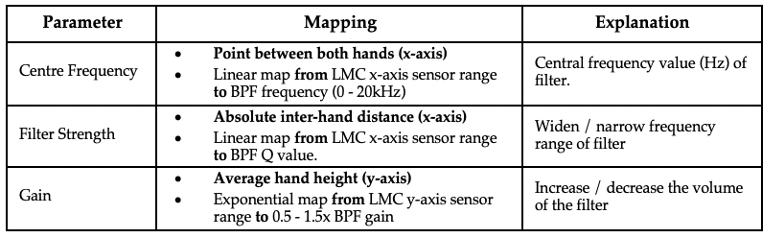
\includegraphics[width=0.8\linewidth]{figures/05-area/areatechnical_param1.png}
    \caption{Band-pass filter parameter mappings}
    \label{fig: areaparams1}
\end{figure}

\begin{figure}
    \centering
    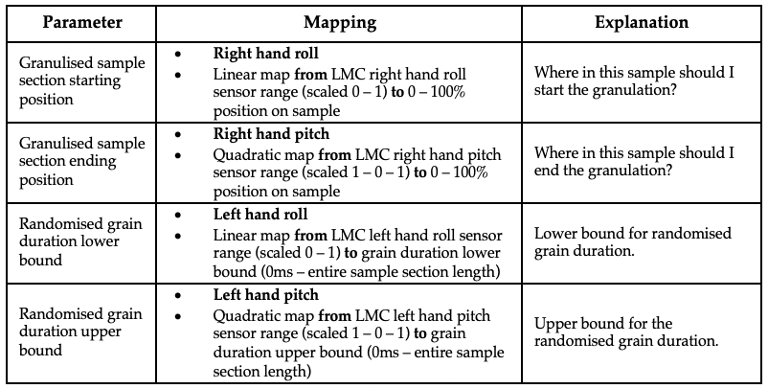
\includegraphics[width=0.8\linewidth]{figures/05-area/areatechnical_param2.png}
    \caption{Granular synthesiser parameter mappings}
    \label{fig: areaparams2}
\end{figure}
When the user decides to end manipulating the sample, they can do so by performing a grab with both hands. Once this happens, the band-pass filter and granular synthesis parameters are frozen for that sample.

\subsubsection{Spatialise}                      \label{sec: area-system-software-spatialise}
\textbf{The spatialise stage} begins once the manipulation stage is ended by the user. The three-dimensional space above the LMC is mapped to the \textit{virtual audio environment}, in which the user is currently listening to the sample that they have recorded. The user can use their right hand to move the sample around the \textit{virtual audio environment}. For an example of the effect this has, moving the hand between the two extremes of the x-axis (left to right) results in hearing the sample move from ear to ear. The spatialise stage is ended by grabbing with the right hand.

Once the spatialise stage has ended, the user has the option to repeat the process 7 more times, allowing for the creation of a \textit{virtual audio environment} comprised of up to 8 spatialised audio samples, or what I refer to as \textit{nodes}. 

\subsubsection{Summary}                         \label{sec: area-system-software-summary}
The audio signal arriving in the two conduction pads in the headphones are the signals of two equidistantly spaced virtual microphones inside the \textit{B-Format virtual audio environment} that decode it into two channels, left and right. Further interaction comes from user head movement which, at all times, is mapped to the revolution of these two virtual microphones around the central point of the \textit{virtual audio environment}. This means if there is a node playing to the left of the user, rotating the head 90° anticlockwise results in the \textit{node} now sounding as if it is in front of the user’s face. This is achieved via the ICST Ambisonics Library \citep{schacher2006} and is elaborated on in the sections \autoref{sec: area-study-results-experiences} and \autoref{sec: area-discussion-aar}, but for now it is worth mentioning that it allows for immersion into a combined \textit{real and virtual audio environment}.

To summarise, the patch can be categorised into having two inputs: audio from the user’s environment and hand gesture, and one output: \textit{the virtual audio environment}. In the background, this audio input is decoded into the \textit{ambisonic palette} (inaudible), which is acted on by the user’s hands to form one audible output: the \textit{virtual audio environment}, which is comprised of up to 8 \textit{nodes}. Through the choice of sensory overlay (bone conduction) and integration of head tracking, this \textit{virtual audio environment} is experienced synchronously with the users’ real, multisensory environment. 



% ---------------------------------------------
\section{Study}                                 \label{sec: area-study}
\subsection{Autobiographical Design}            \label{sec: area-study-abd}
Originally, the study was planned for late March and would involve several user interaction studies. However, due to the UK lockdown in response to the unfolding COVID-19 pandemic, this was postponed until later in the year. Instead, I investigated the system using an autobiographical design method, framing it as a hypothesis study to better understand relationships between virtual and real environments, in the hope of developing a practice-led method for creating and researching multisensory augmented reality experiences. 

Autobiographical design is defined as “design research drawing on extensive, genuine usage by those creating or building the system” \citep{neustaedter2012}. Neustaedter and Sengers define “genuine usage” here to mean that changes are “based on the true needs of the researchers, rather than them pretending to have needs expected of target users”.

Due to the lockdown, and therefore inability to conduct in-person user-tests, this research method was beneficial as I was spending large amounts of time with the system. Moreover, there are several suggested requirements of employing this research method that Neustaedter and Sengers highlight that are true of the \textit{area\textasciitilde{}} system:
\begin{itemize}
    \item The existence of a genuine usage of the system
    \item The system being already developed
    \item The ability for fast tinkering 
    \item Record-keeping of the design process
    \item Long-term usage of the system
\end{itemize}
Furthermore, as AR technology moves towards being a component of future general personal computing, there is a need for first-person research methods that take into consideration the effects of prolonged system usage as well as the arising relationship between user and system \citep{desjardins2018}. Moreover, these methods have been found to be specifically relevant to wearable systems \citep{cecchinato2017}.

A disadvantage of using autobiographical design as a research method is its inability to establish generalisability (also the case with ethnography, case studies and participatory workshops), which is why I still intend to conduct wider usability studies in the future.

\subsection{Design}
                                                \label{sec: area-study-design}
The study was designed as a cycle, in order to promote fast tinkering, record-keeping, and long-term usage in line with autobiographical design guidelines. 
\begin{enumerate}
    \item Over three sessions, ideally during the same week, the system is used with a logbook at hand in order to facilitate record-keeping of hardware setup, \textit{node} manipulation and completed \textit{real and virtual audio environment} listening experience remarks.
    \item After each session, the notes are formalised into a database and categorised as “user experience remarks” or “improvement remarks” (subject to increase in categories). 
    \item At the end of the week, the three sessions’ notes are summarised into a “check-in” document, where user experience remarks are collated, and improvement remarks are further categorised into lists pertaining to the area of the system that needs improvement or change.
    \item Those changes are then made to the system and the cycle restarts.
\end{enumerate}

\subsection{Results}                            \label{sec: area-study-results}
\subsubsection{Hardware Location}               \label{sec: area-study-results-hwloc}
I have observed that an environment with a lower noise floor is desirable and have implemented a normaliser to deal with re-recording loud background / ambient noises during successive \textit{node} recording. I found myself basing the choice of microphone placement on what I wanted the \textit{virtual audio environment} to sound like. Since the system uses an ambisonic microphone, consideration of the spherical 360° field of the microphone would lead to a richer \textit{ambisonic palette} and subsequent \textit{virtual audio environment}.

Two sessions were based outdoors and involved natural sounds such as birds, trees and wind, as well as passing cars. One of the sessions was inside and took place at the same time my partner was on a Zoom call, and therefore the \textit{ambisonic palette} was invariably based on her speech and my movement and action inside the room. I want to look into placing the microphone inside bushes, trees, etc. rather than in open spaces to explore aesthetically the \textit{virtual audio environment} that arises from such placement. Furthermore, the relationship between \textit{real and virtual audio environment} would be quite different. Through their ears, the user would be rooted in their position in the environment, but because of the inherent blend between hearing and bone conduction, they would simultaneously experience the sonic environment of the bush mediated by the Max MSP patch.

\subsubsection{Experiences}                     \label{sec: area-study-results-experiences}
The system takes considerable time to set up, especially when documenting with video, audio, and notes. This process could certainly be streamlined further. Overall, I was pleased with the sound quality; the microphone picks up the environment very clearly. However, I remarked that the manipulation stage could feature more interesting real-time auditory effects on the \textit{nodes}. The blending of \textit{real and virtual audio environment} is achieved well via the bone conduction headphones and there was a subconscious registration via the head-tracking that gave me the very real impression that there was a 3D environment of \textit{nodes} around my body.

The IMU on the bone conduction headphones sometimes provides erratic and erroneous data, leading to accidental revolutions of the \textit{virtual audio environment} around the head. Despite technical difficulties such as this, in one autobiographical design session, when I took the headphones off, I wrote that “I felt like I'd been disconnected from something” and that “my senses felt heightened before I took them off, not only to the \textit{virtual audio environment}, but now more sensitive to the audio content of my real environment.

If I managed to capture an infrequent environment sound, such as a particular bird call, or a sentence of spoken word, the fact that the patch is set up to loop the samples gave a certain permanence to that otherwise impermanent sound. On multiple occasions I could not tell if the sounds of birds I was hearing originated from a \textit{node} or from within a tree.

\subsubsection{Arising Interactions}            \label{sec: area-study-results-arisingints}
The maximum sample length is currently 28 seconds, but I have found myself mainly sticking to shorter loops, creating quite repetitive and rhythmic sequences. I remarked that grains from the synthesiser sounded like a permanent record of my gestures’ effect on the environment. I liked the playfulness of being able to record a sound from a certain location in my \textit{real audio environment} and place it in different location in my \textit{virtual audio environment}.

Despite the wearable hardware being wireless, hand interaction with the \textit{area\textasciitilde{}} system is inherently limited to being in range of the LMC (often placed on a table). I found myself wanting to be able to move around my environment whilst being able to record new nodes and hear existing nodes move relative to my body position.

Overall, the results from my autobiographical design method have shown that \textit{area\textasciitilde{}} is an effective tool for examining the combinatorial relationship between real and virtual environments. Despite the system’s hardware setup requiring some further work to allow for quicker start up and more accurate head tracking, it has provided me with novel aesthetic experience through:
\begin{itemize}
    \item The blending of \textit{real and virtual auditory environments} to create a third, augmented environment that was greater in experiential nature than the sum of its parts (not simply a combinatorial layering)
    \item The ability to spectromorphologically manipulate sounds in real-time in this third environment with the body
    \item The potential for creating believable illusions of real-world sound sources from these manipulated and spatialised virtual sounds.
\end{itemize}

% ---------------------------------------------
\section{Discussion}                            \label{sec: area-discussion}
\subsection{Audio Augmented Reality}            \label{sec: area-discussion-aar}
In \autoref{sec: literature-interface-process}, I detailed the importance of the relationship between real and virtual environments in the definition of AR systems. As a medium for creating computational art, the three specifications outlined by \citep{azuma1997} still hold true and should be discussed in the creation of such art or the development of their interactive systems of composition e.g. \textit{area\textasciitilde{}}.
\begin{enumerate}
    \item Combines real and virtual
        \begin{itemize}
            \item Using bone conduction headphones means that the user’s unmediated perception of the environment is allowed to continue without interference, allowing the effective combination of real and virtual environments.
        \end{itemize}
    \item Interactive in real-time
        \begin{itemize}
            \item The system is made interactive in real-time through the gestural mappings (both head and hand) to sound effect parameters, and the perception of those effects through the mediating sensory display (bone conduction headphones).
        \end{itemize}
    \item Registered in 3-D
        \begin{itemize}
            \item The \textit{area\textasciitilde{}} system is registered in 3-D via the IMU data allowing for the mapping of head movement to \textit{virtual audio environment}. 
            \item The mapping of hand movement (in the recording stage) to the spatial location recorded in the ambisonic palette (detailed in \autoref{sec: area-system-software}), also contributes to the notion that the \textit{virtual audio environment} and real audio environment are aligned.
        \end{itemize}
\end{enumerate}

\subsection{Interaction}                        \label{sec: area-discussion-interaction}
The tables of parameter mappings shown in \autoref{sec: area-system-software-manip} may seem like a chaotic mess, however, time has been spent making these mappings intuitive. For example, the representation of volume to a vertical scale corresponds with findings that non-musicians are relatively competent at attributing the size of air-gestures to heightened musical dynamics \citep{godoy2006,caramiaux2010}. As for the band-pass filter’s horizontal pitch mappings, this is mainly based on the visual representation of frequencies on a horizontal scale often found in the user interface of such filters. Nevertheless, it is pertinent to mention that field of psycho-musicology research \citep{timmers2016} finds a correlation between pitch representation and horizontal space i.e. lower pitch to the left, higher pitch to the right. Although this is often attributed to the internalised representation of horizontal pitch on pianos by keyboard-playing musicians \citep{lidji2007,rusconi2006}, it has been found that this effect also propagates in non-musicians \citep{weis2016}. This is also found to be the case in the “Playing air-instruments” study carried out by Godøy, Haga, and Jensenius \citeyearpar{godoy2006}.

In contrast, interaction with the granular synthesiser is not made to be intuitive; instead, I have opted to hide or black-box the interaction through a mix of linear and quadratic mappings on each hand. This is in order to stir curiosity in the user and induce play, as found in \autoref{sec: area-study-results-arisingints}, but also to be tested in wider user studies, “I remarked that grains from the synthesiser sounded like a record of my gestures’ effect on the environment”.

Indeed, whilst outlining the material epistemologies of digital music instruments (DMIs), \citep{magnusson2009} describes black-boxed DMIs as containing  “knowledge of its inventors, which means that the users of the instrument do not need to have a deep knowledge of its internal functions”, furthermore clarifying that there is a “continued oscillation between a mode of conceptual (system design) engagement with the instrument and [an] embodied (performative) relationship with it”. This ‘oscillation’ displays, in turn, an underlying synergy between DMI development and the autobiographical design process, perhaps due to the similarities in requirements of the processes outlined in \autoref{sec: area-study-abd}. This synergy has led to the use of ABD in the development of many DMIs and interactive music systems \citep{kiefer2020,martin2017,turchet2018,unander-scharin2014}.

\subsection{Computational Art}                  \label{sec: area-discussion-computationalart}
\begin{figure}
    \centering
    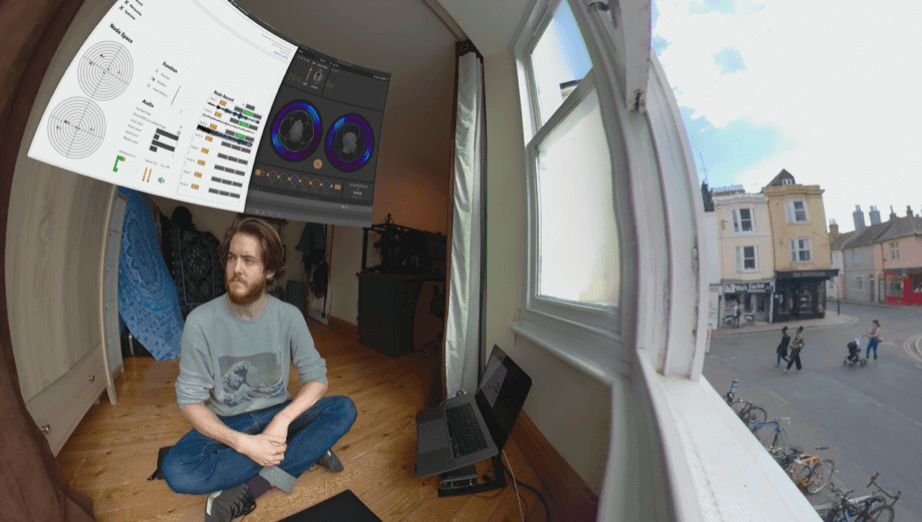
\includegraphics{figures/05-area/areafuturedoc.png}
    \caption{\textit{area\textasciitilde{}} 360° video and ambisonic documentation \citep{bilbow2020}}
    \label{fig: areafuturedoc}
\end{figure}
As a system for creating computational art in the form of in-situ AAR experiences, \textit{area\textasciitilde{}}’s artistic output is firstly a real-time experience. In order to document these experiences of the system however, I have included the automated recording and saving of both the \textit{ambisonic palette} (the ambisonic recording of the real audio environment), and the users \textit{virtual audio environment} as separate B-Format .wav files in the project directory. These separate B-Format .wav files could be merged and decoded from B-Format to any number of speakers for a multi-channel installation of field recordings or manipulations of environments made with \textit{area\textasciitilde{}}. This also leaves open the potential for \textit{area\textasciitilde{}} to be used as a compositional tool, with potential applications in sound art and soundscape composition.

I also chose to merge and decode a set of these recordings to binaural ambisonic format, and have time-synced this recording with a 360° video and a screen recording of the patch that was taken during the system’s use. This allows my performance of the virtual audio environment to be experienced second-hand with headphones. Dragging the screen in different directions with mouse/touchscreen emulates hearing the difference in environment if I moved my head in those directions. Optionally, an inexpensive smartphone VR headset (£5 - £15) can be used to heighten the interactivity of the experience. A screenshot of the 360° video \citep{bilbow2020} is shown in \autoref{fig: areafuturedoc}. The potential for users’ experiments with \textit{area\textasciitilde{}} to be captured and re-experienced interactively could have interesting applications, effectively allowing users to explore each others’ lived aural experience of the system.

% ---------------------------------------------
%\section{Future Research}                       \label{sec: area-future}
%
%\subsection{Devising a practice-led method}     \label{sec: area-future-method}
%The  novel experiences that emerged from the results of the study into the uses of AR as a medium for computational art have encouraged me to devise a practice-led method for researching multisensory AR (MSAR). It begins with the ideation of an MSAR Experience (which describes a possible human-to-sense interaction). These are classed as Snippets, Scenes, and Spaces depending on the number of senses engaged, sensory intensity, and interaction size. The hardware and software that enable the experience are classed as MSAR Instruments and MSAR Environments respectively. Instruments are categorised into Wearable, Tangible and Situated Instruments. This taxonomy will eventually aid not only in the creation, but in the evaluation of future MSAR Experiences. 
%
%\subsection{Project North Star}                 \label{sec: area-future-pns}
%As mentioned in \autoref{sec: area-study-results-arisingints}, the ability to move around whilst recording nodes could address the rigidity of the hand gestures being tethered to the Leap Motion Controller, which was often placed on a table, but is inherently connected to the laptop. One way of achieving this would be changing the wearable portion of the hardware. Instead of the IMU paired with bone conduction headphones, I could move towards the use of a head mounted display (HMD) paired with the bone conduction headphones. This would most likely be the open-source AR HMD design by Leap Motion: Project North Star \citeyearpar{leapmotion2018}, for which there is a large community of makers. The HMD integrates the same LMC (hand tracking), as well as an Intel RealSense T261 for inertial measurement data (body position tracking, not just head). 
%
%The headset being used with the Project Esky software toolkit \citep{rompapas2020} to resize virtual objects in a demo is shown in Figure 9. The headset requires a computer to power it, although a portable compute pack for the HMD is in development by CombineReality \citeyearpar{combinereality2020}. Regarding \textit{area\textasciitilde{}}, the use of body position tracking rather than just head orientation tracking, and the move from a desk-placed LMC to head-mounted, opens avenues for different and potentially more interactive gestures i.e., allowing for the re-manipulation of, or interacting with existing nodes in a larger environment. Rather than feeling like they were rooted to an instrument, the system would move towards being more of an extension of the performer, and with this, new aesthetic experiences of real and virtual space would be explored, for example enabling the recording of previously inaccessible environments: in the city centre, or by the beach, where the user would not be able to set up a table. 
%
%\subsection{Multisensory area(s)\textasciitilde{}}  \label{sec: area-future-multisensory}
%In broader terms of my practice-led method, Project North Star provides an open-source Wearable Instrument, and through preliminary engagements, has shown that it is an extremely malleable platform for creating multisensory AR Experiences, as well as mounting further Wearable MSAR Instruments.

%I envisage the future of \textit{area\textasciitilde{}} to not only include visualisations of nodes, but haptic interactions with nodes. I see no reason why olfactory displays of nodes couldn’t be integrated too, either via North Star mounted injection, or in zones of interaction in a multisensory \textit{area\textasciitilde{}} installation or performance space. This would allow for a more “modalities-encompassing” \citep{schraffenberger2016} approach to understanding nuances in the relationship between the real and virtual environments of AR when it is used as a medium for expressive computational art.